\chapter{Conclusão}

Desde a confirmação e descoberta das ondas gravitacionais, muito se falou sobre este assunto, consequentemente muitos estudos voltados a esta área vieram a tona. Mesmo assim, poucos estudos foram feitos mesclando o uso de Machine Learning com as ondas gravitacionais. Diante disto, esta pesquisa se caracteriza como uma grande contribuição nesta areá de pesquisa que aos poucos esta atraindo mais visibilidade. 

Nesta pesquisa foi empregado um comitê de redes neurais com hiperparâmetros rigorosamente ajustados e produzido uma saída que retorna uma estatística de classificação equivalente à uma função de pertinência inferida de que os dados contêm um sinal de onda gravitacional, mostrando que o método empregado neste trabalho pode, em princípio, ser usada para pesquisar diretamente sinais GW nos dados, em tempo de pesquisa teoricamente, substancialmente mais rápido do que as abordagens com Deep Learning e filtragem correspondente.

Devido a simplicidade da arquitetura das redes neurais desenvolvidas, torna possível este método capaz de ser reproduzido em ambientes computacionais mais simples, que estão ao alcance do hardware comercial disponível hoje. Além disso, a escalabilidade intrínseca desta metodologia pode superar e abranger o espaço de parâmetros de fusão de buracos negros e ser aplicado a outros tipos de fusão, como sinais de fusão de binários de estrelas de nêutrons e fusão de estrelas de nêutrons com buracos negros. 

Essas capacidades podem permitir pesquisas rápidas e automatizadas de GW em qualquer ambiente, cobrindo milhões ou bilhões de modelos em toda a gama de espaço de parâmetros que está além do alcance dos algoritmos existentes. Portanto, esperamos que essa abordagem aumente a profundidade e a velocidade do algoritmo desenvolvido, permitindo pesquisas online em tempo real após ser treinado com bancos de modelos de milhões ou bilhões de formas de onda.

Os resultados obtidos seguindo a metodologia descrita neste trabalho além de ótimos, abrem um leque de possibilidades de descobertas através deste método. Uma das descobertas preliminares foi a estimativa do tempo de fusão-ringdown de todas as fusões usadas nesta pesquisa, o qual, o LIGO somente tem conhecimento de metade delas. Também foi descoberto um Plator presente em todas os resultados desta pesquisa, na Figura~\ref{fig:scoreHLPlator} é possível notar que após o decaimento do score ao final da fusão dos buracos negros existe uma pequena ondulação que possivelmente pode ser a reverberação pós fusão dos dois buracos negros. Estes estudos estão em andamento e serão descritos em um artigo subsequente. Diante disto, estas revelações demostram a grande aptidão desta pesquisa em desvendar novas informações sobre as ondas gravitacionais.

\begin{figure}[H]
\centering
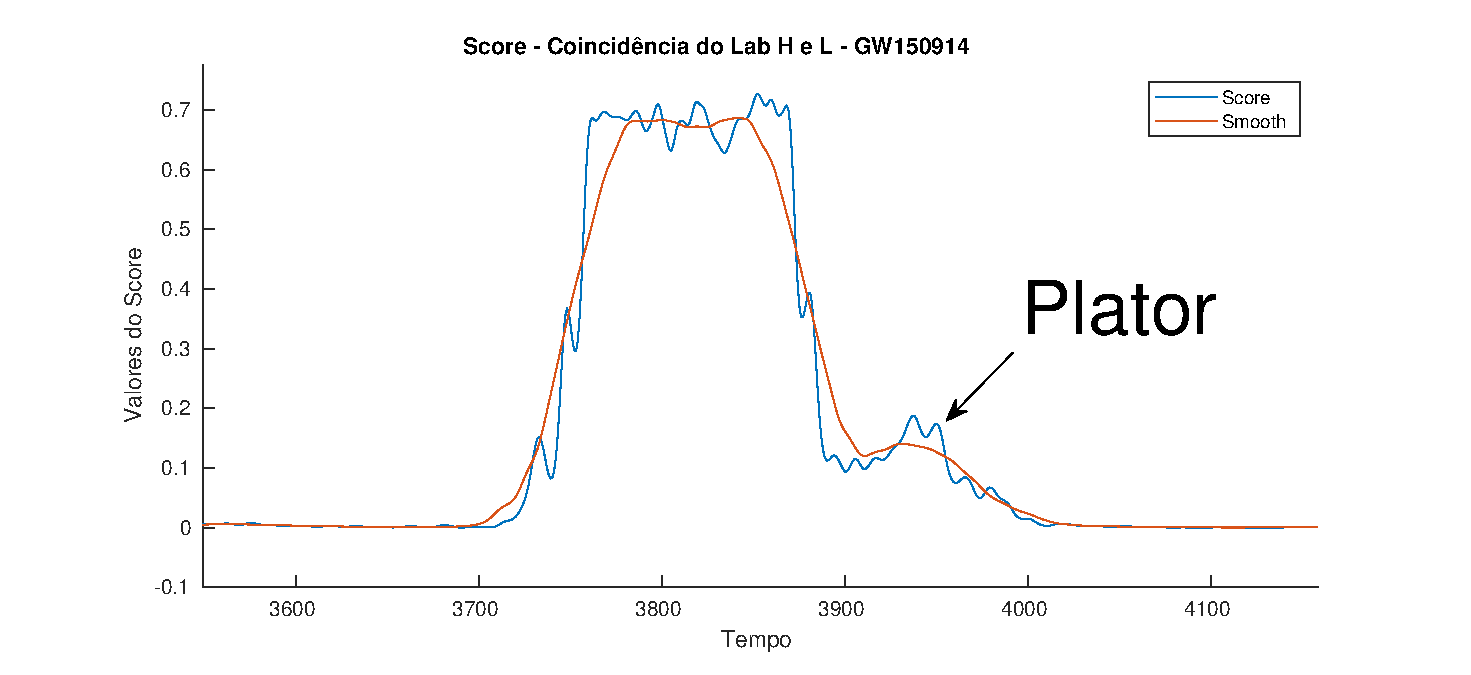
\includegraphics[width=1\textwidth]{figuras/GW150914_LabHL_plator.eps}
\caption{Zoom do resultado da coincidência entre os laboratórios H1 e L1 para a GW150914 com a marcação do Plator.}
\label{fig:scoreHLPlator}
\end{figure}

Além do mais, os resultados apresentados nesta pesquisa fornecem um forte incentivo para estender a metodologia para a possibilidade de estimativa de parâmetros assim como em~\cite{PhysRevD.97.044039,GEORGE201864}. Futuramente, será investido mais esforço no ajuste de hiperparâmetros e inclusão de novas formas de ondas que abrangem diversos parâmetros de fusões, ao ponto de superar a sensibilidade das pesquisas de Deep Learning e matched-filtering. Ademais, será pesquisado a estimação de parâmetros juntamente com a detecção de sinais nos dados do LIGO, tornando a detecção rápida com a estimativa de parâmetros igualmente rápida fundamental para a astronomia de ondas gravitacionais.

Essas considerações fornecem motivação suficiente para desenvolver e implantar novas abordagens nesta área de pesquisa afim de produzir um pipeline de detecção de sinais de GW único, simples e computacionalmente eficiente que unifica a detecção em tempo real de GW e a estimativa de parâmetros, em que, qualquer um posso usar e desenvolver novas pesquisas, fazendo deste um método de pesquisa competitivo.

Esperasse que esta nova abordagem penetre na comunidade científica e sirva como um passo fundamental para permitir observações em tempo real de sinais GW, fornecendo alertas imediatos para acompanhamento após eventos de GW. Também almejasse que esta nova metodologia para processar sinais em dados ruidosos seja útil em muitas outras áreas, tornando essa metodologia muito promissora para vários campos de pesquisa. Fazendo deste trabalho o alicerce para integralizar diversos setores de especialização para permitir e acelerar descobertas científicas.

No geral, esta pesquisa tem potencial para se tornar uma ferramenta útil de pesquisa para a analise de GW, mas há um esforço substancial de pesquisa e desenvolvimento para alcançar isso.